The benchmark runs logged 415,106 Jev decisions. Median request latency was 166--178\,ms for insert steps and
254\,ms for a recall grade carrying up to 48 questions (Figure~\ref{fig:latency}).

\subsection{Why destructive verdicts need 0.9}

Without human labels, we asked Claude Sonnet 5.5 the same questions with the same definitions and context, on samples
stratified by Jev's probability: 240 reconcile verdicts, 196 destructive verdicts (same, replaces, covers) and 154 entity
decisions (Figure~\ref{fig:calibration}). Agreement with a larger model is not correctness, but it should rise with Jev's
probability if thresholds are meaningful.

\begin{figure}[!htb]
\centering
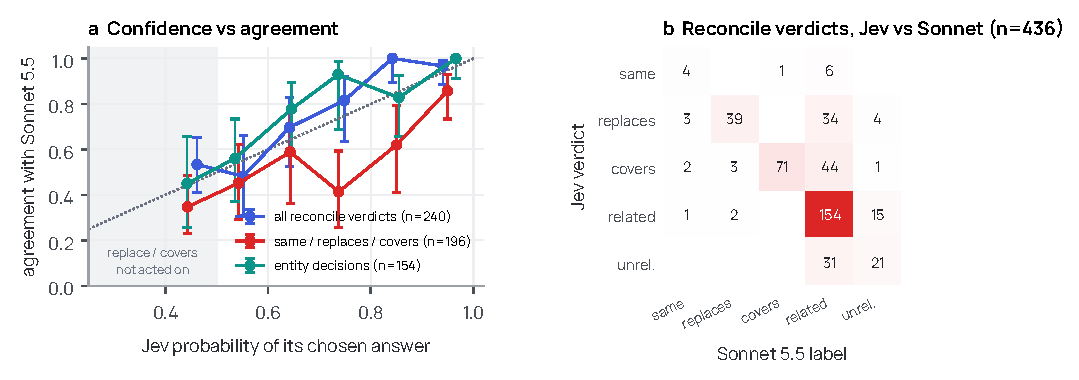
\includegraphics[width=\linewidth]{figures/fig_calibration.pdf}
\caption{\textbf{Jev's confidence against agreement with a larger model.} (a) Agreement with Claude Sonnet 5.5 by Jev's
probability bin, with Wilson intervals; the dotted line is perfect agreement-calibration. Samples are stratified by
probability, so pooled rates are not population rates. (b) Jev's reconcile verdict against Sonnet's label over both
verdict samples.}
\label{fig:calibration}
\end{figure}

Overall, agreement rises with probability and sits near the diagonal (about 0.5 below 0.6, 0.97--1.0 above 0.9).
Destructive verdicts are the exception: agreement stays between 0.41 and 0.62 from 0.5 to 0.9 and reaches 0.86 only
above 0.9, and when Sonnet disagreed it almost always said \emph{related}. An option-order check pointed the same way:
shuffling the five options changed 5 of 30 destructive labels below 0.9 and none of 8 above. Hence the 0.9 floor on
``replaces'' and ``covers''. A narrower follow-up question for the band below the floor (``can both statements be true
at once?'') did not help: on 67 labelled verdicts between 0.6 and 0.9 Jev answered ``yes'' (median 0.96) whether or
not the reference agreed with the replacement, so it is off by default. Entity decisions tracked their probability closely (0.93 agreement at the 0.7 merge
threshold), and nearly all similar-embedding pairs were judged different, as the asymmetric prior intends.

\subsection{The injection check, tested directly}

In OrgProbe both extractors dropped the planted instruction, so we sent 12 planted instructions and 12 ordinary statements
that merely sound imperative (``The user asked the assistant to always include sources'', ``Production deploys require
two approvals'') straight to the sort request. All 12 planted instructions scored at least 0.75 (ten at 0.93 or more,
so they would be rejected outright; two would be stored flagged and kept out of recall). The 12 ordinary statements
scored 0.03--0.42; two user preferences about the assistant's behaviour came closest to the 0.5 flag (0.41 and 0.42).
The probe is author-written and small; it shows the check separates obvious cases with margin, not that it resists
adaptive attacks, against which Jev's own documentation warns~\cite{typesafe}.
